\setAuthor{Jaan Kalda}
\setRound{lahtine}
\setYear{2018}
\setNumber{G 3}
\setDifficulty{3}
\setTopic{Elektriahelad}

\prob{Ring}
Traadist, mille ühe detsimeetri takistus on üks oom tehakse ring ümbermõõduga kuus detsimeetrit. Iga detsimeetri järel märgitakse punktid $a, b, \ldots, f$. Punktide $a$ ja $e$ vahele ühendatakse patarei pingega \SI{7}{V}, punktide $d$ ja $f$ vahele ampermeeter ning $d$ ja $b$ vahele voltmeeter. Punktid $f$ ja $b$ ühendatakse samast traadist lõigatud kahe-detsimeetrise traadijupiga. Leidke ampermeetri ja voltmeetri näidud.




\hint
Ülesandes tasub selgelt skeem välja joonistada. Voolude ja pingete arvutamiseks võib $d$ ja $f$-i ühe punktina kujutada.\solu
\begin{wrapfigure}[11]{r}{0.4\textwidth}
	\vspace{-20pt}
	\begin{center}
		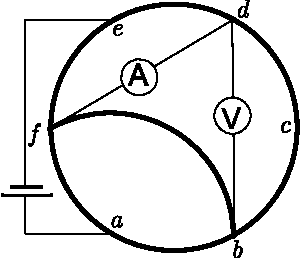
\includegraphics[width = 0.4\textwidth]{2018-lahg-03-yl.pdf}
	\end{center}
\end{wrapfigure}

Koostame joonisel kujutatud ekvivalentskeemi. Kuna ampermeeter ja voltmeeter on ideaalsed, võime need vastavalt traadiga asendada ja skeemist kõrvaldada. Voltmeeter on kinnitatud punktide $b$ ja $d$ vahele, mille vahel on takistus $2R$. Kirhoffi vooluseaduse tõttu näitab ampermeeter punktist $d$ punkti $e$ kaudu väljuva voolu ja punkti $b$ kaudu siseneva voolu vahet. Niisiis, punktide $a$ ja $d$ (või ekvivalentselt $f$) vaheline takistus koosneb kahest rööbiti ühendusest ja ühest jadamisi ühendusest. Peale takistuste taandamist leiame, et nende vaheline takistus on $2R/3$. Punktide $d$ ja $e$ vaheline takistus koosneb kahest rööbiti takistusest kogutakistusega $R/2$. Skeemi kogutakistus on seega $7R/6$. Voolutugevus läbi patarei on $I_0 = \mathcal{E}/(7R/6) = 6\mathcal{E}/(7R)$ ning see jaguneb punktist $a$ vasakpoolse ja parempoolse haru vahel vastavate harude takistuste suhte järgi vahekorras 2:1, st paremasse harru läheb vool $I_0/3 = 2\mathcal{E}/(7R)$. Edasi voolab punktist $b$ vool võrdselt punktidesse $f$ ja $d$ ning seega langeb voltmeetrile pinge $U = 2R\mathcal{E}/(7R) = 2\mathcal{E}/7=\SI{2}{V}$. Kuna punkti $e$ siseneb vool võrdselt harudest $d$ ja $f$, siis ampermeetri näit on $I_A = I_0/2 - \mathcal{E}/(7R) = 2\mathcal{E}/(7R) = \SI{2}{A}$.\probend